\documentclass{beamer}

\usetheme{Montpellier}
\usepackage{tikz}

\definecolor{beamer@blendedblue}{rgb}{0.3,0.5,0.6}

\setbeamercolor{normal text}{fg=black, bg=white}
\setbeamercolor{alerted text}{fg=red}
\setbeamercolor{example text}{fg=green!50!blue}

\title{Virtual Reality for Sensor Data Analysis}
\subtitle{SW-Projekt SS 2017 Gruppe 5.1}
\author{Gero Birkh\"olzer \and Johannes Blank \and Alexej Gluschkow \\ \and Fabian Klopfer \and Lisa-Maria Mayer}
\date{Zwischenpr\"asentation am 12. Juni 2017}



\addtobeamertemplate{frametitle}{}{%
\begin{tikzpicture}[remember picture,overlay]
\node[anchor=north east,yshift=2pt] at (current page.north east) {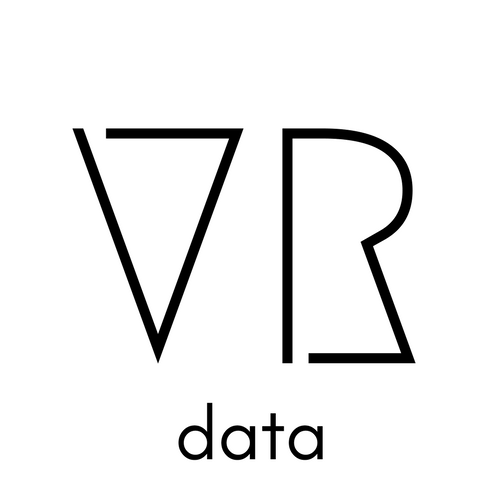
\includegraphics[height=0.8cm]{logo.png}};
\end{tikzpicture}}


\begin{document}


\frame{\titlepage}



\begin{frame}
  \frametitle{Inhalt}
  \tableofcontents%[hideallsubsections]
\end{frame}


\section{Einleitung}

\subsection{Aufgabenstellung}

\begin{frame}
\frametitle{Einleitung}
\framesubtitle{Aufgabenstellung}
\begin{itemize}
	\item Visualisierung von mindestens einem Sensorwert (z.B. Temperatur) in Abh\"angigkeit von seiner Position.
	\item Verschiedene Visualisierungsm\"oglichkeiten der Sensordaten.
	\item Visualisierung in einer vorgefertigten 3D-Umgebung, basierend auf der Originalumgebung.
\end{itemize}
\end{frame}

\subsection{Idee} %Requirements

\begin{frame}
\frametitle{Einleitung}
\framesubtitle{Idee}
\begin{itemize}
  \item Aufzeichnen von Daten mit der App.
  \item Positionstracking \"uber das Smartphone.
  \item Anzeigen der aufgenommenen Daten in der WebVR Umgebung.
\end{itemize}
\end{frame}

\subsection{Umsetzung} %SDD

\begin{frame}
\frametitle{Einleitung}
\framesubtitle{Umsetzung}
\begin{itemize}
	\item Aufspaltung in zwei Teile: \pause
  \begin{enumerate}
    \item App f\"ur die Verbindung zum Sensor, Ortsbestimmung und Datenspeicherung.
    \item Webanwendung zur Darstellung der Daten und der 3D-Umgebung.
  \end{enumerate}
\end{itemize}
\end{frame}

%\begin{frame}
%\frametitle{Composite Diagram}
%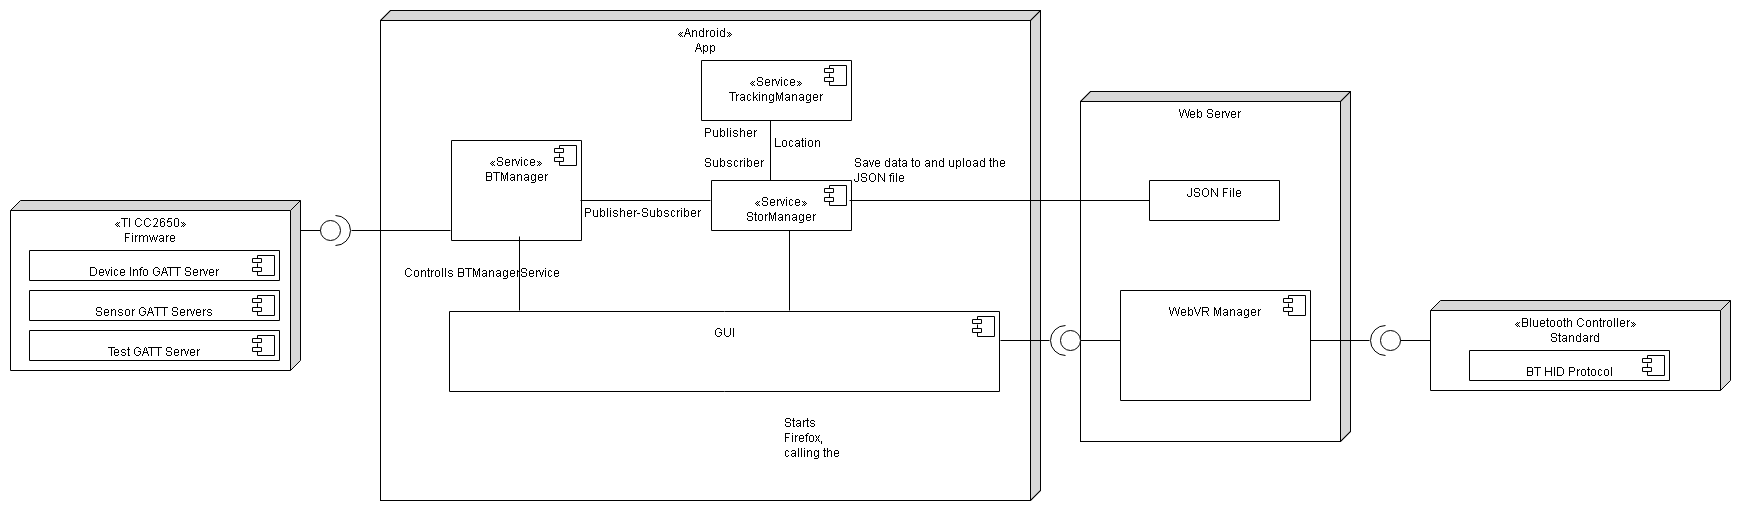
\includegraphics[width=\textwidth]{../doc/SDD/pics/composite_app.png}
%\end{frame}


\section{GUI}

\begin{frame}
\frametitle{GUI}
\framesubtitle{Bisherige Funktionen}
\begin{itemize}
  \item Splash Screen beim Starten der App
  \item Grundlegende Strukturierung durch Tableiste
  \item Starten des Browsers, um Webanwendung auszuf\"uhren
  \item Sendet Intent an den Bluetooth-Manager, um Scan zu starten und Live-Data anzuzeigen.
\end{itemize}
\end{frame}

\begin{frame}
\frametitle{GUI}
\framesubtitle{N\"achste Schritte}
\begin{itemize}
  \item Tab-Activities zu Fragments umwandeln
  \item LiveData in RecordActivity einbinden
  \item SettingsActivity: Tracking- und Bluetooth-Funktionen sinnvoll integrieren
  \item Layout vereinheitlichen
\end{itemize}
\end{frame}


\section{Bluetooth-Manager}


\begin{frame}
\frametitle{Bluetooth-Manager}
\framesubtitle{Bisherige Funktionen}
\begin{itemize}
  \item Scannen nach TI CC2650 MCU(s)
  \item Verbinden zum GATT Server eines TI CC2650 MCU
  \item Anzeigen erhaltener Sensordaten in einer Live-Ansicht
  \item Senden der Sensordaten (via LocalBroadcastManager) bzw. starten des IntentService
\end{itemize}
\end{frame}

\begin{frame}
\frametitle{Bluetooth-Manager}
\framesubtitle{N\"achste Schritte}
\begin{itemize}
  \item Debuggen (insbes. Scan)
  \item Code kommentieren
\end{itemize}
\end{frame}


\section{Storage-Manager}

\begin{frame}
\frametitle{Storage-Manager}
\framesubtitle{Bisherige Funktionen}
\begin{itemize}
  \item Speichert den letzten Empfangenen Intent
  \item Skaliert die Daten und schreibt diese in eine JSON-File
  \item Bindet Tracking-Manager, noch kein Datentransfer von diesem
\end{itemize}
\end{frame}

\begin{frame}
\frametitle{Storage-Manager}
\framesubtitle{N\"achste Schritte}
\begin{itemize}
  \item Webserver einrichten
  \item Dateien auf Webserver hochladen
  \item Positionsdaten einbinden
  \item Code kommentieren
\end{itemize}
\end{frame}

\section{Tracking-Manager}

\begin{frame}
\frametitle{Tracking-Manager}
\framesubtitle{Bisherige Funktionen}
\begin{itemize}
  \item Grobe Positionsbestimmung durch GPS oder Networkprovider
  \item	Genauere Positionsbestimmung durch Trilateration von WLAN-Accesspoints
  \item	Abstandsbestimmung duch RSSI
  \item	APs k\"onnen individuell konfiguriert und f\"ur das Tracking selektiert werden.
\end{itemize}
\end{frame}

\begin{frame}
\frametitle{Tracking-Manager}
\framesubtitle{N\"achste Schritte}
\begin{itemize}
  \item TESTEN\\
  		(Raum w\"ahlen, ggf. APs installieren und konfigurieren)
  \item Verbesserungsm\"oglichkeiten:
  		\begin{itemize}
  		\item	Smoothing der RSSI-Daten
  		\item	Kombination mit Accelerometer und Gyrometer Daten
      \item Code kommentieren
  		\end{itemize}
\end{itemize}
\end{frame}


\section{Webanwendung}

\begin{frame}
\frametitle{Webanwendung}
\framesubtitle{Bisherige Funktionen}
\begin{itemize}
  \item Umstellung auf stereoskopische 3D-Ansicht m\"oglich
  \item Rudiment\"are 3D-Welt
  \item Bewegung mit dem Gamepad m\"oglich
  \item 2 verschiedene Visualisierungsm\"oglichkeiten der Daten
  \item Umstellung der Visualisieren mit Gamepad m\"oglich
\end{itemize}
\end{frame}

\begin{frame}
\frametitle{Webanwendung}
\framesubtitle{N\"achste Schritte}
\begin{itemize}
  \item Modellierung des Raumes in Blender
  \item Code kommentieren
\end{itemize}
\end{frame}

\end{document}
